\section{Univariate Data}

\textbf{07.03.2023 - Lecture 1 - EDV1}


Let's say we are measuring $x$. $i$ substring denotes the measured value of $x$.

$x_i$: $i^{th}$ measurement value in chronological order.

$x_{(i)}$: $i^{th}$ measurement value in a ranked (or sorted) order as in:

$$x_{(1)}<x_{(2)}<x_{(3)}<x_{(4)}$$

\textbf{Mean value of a data set:}

$$\bar{x} = \frac{1}{N} \sum_{i=1}^{N} x_i$$

\textbf{Property of the mean value:}

$$x_1 - \bar{x}; x_2 - \bar{x}; ... ; x_n - \bar{x}$$

$$\sum_{i=1}^{n} (x_i - \bar{x}) = \sum_{i=1}^{n} x_i - \sum_{i=1}^{n}\bar{x} = n\bar{x} - \bar{x}n = 0$$

median, $\alpha$ - quantile

sorted dataset $$x_{(1)} \le x_{(2)} \le x_{(3)} \le x_{(4)}$$

\textbf{Example: $n = 11$}

The on that is right in the middle, the center of the sorted data set, is called the median. If the size of the data set is an even number, then the median is:

$$\tilde{x} = \frac{x_{0.5n}+x_{0.5n+1}}{2}$$

\subsection*{Measures of Dispersion or Variance}

Range:
$$R = {max} - {min} = x_{(n)} - x_{(1)}$$

\textbf{Dispersion:} Is the deviation of a value within the data set, from the mean value of the data set.

$$\frac{1}{n} \sum_{u=1}^{u}(x_{(i)} - \bar{x})$$

\textbf{Mean absolute deviation (MAD):}

$$ MAD = \frac{1}{u} \sum_{i=1}^{u} |x_{(i)} - \bar{x} |$$

\textbf{Standard Deviation:}

$$ s = \sqrt{\frac{1}{N-1} \sum_{i=1}^{N}(x_{(i)} -\bar{x})^2} $$

$$\sum_{u=1}^{u}(x_{(i)} - \bar{x}) = 0 $$

The number of independent terms is called "\textit{degree of freedom}". Standard deviation is sensitive to outliers.

\subsection*{Interquantile Range (IQR)}

$$IQR = Q(0.75) - Q(0.25)$$

\textbf{\textit{Note:}} IQR contains \%50 of all values.

\subsection*{Graphical Methods}

\textbf{Histogram:}

\begin{center}
	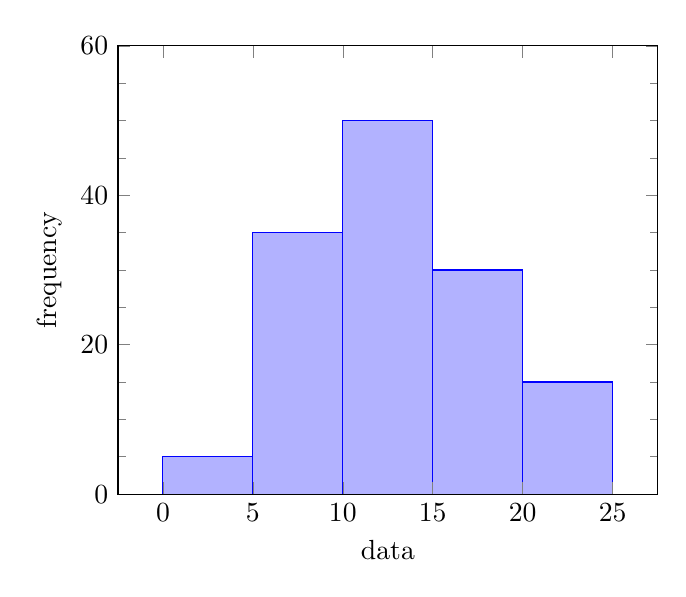
\begin{tikzpicture}
		\begin{axis}[
			ymin=0, ymax=60,
			minor y tick num = 3,
			area style,
			xlabel=data,
			ylabel=frequency
			]
			\addplot+[ybar interval,mark=no] plot coordinates { (0, 5) (5, 35) (10, 50) (15, 30) (20, 15) (25, 0) };
		\end{axis}
	\end{tikzpicture}
\end{center}

Best class width for a histogram is:

$$\boxed{2*IQR*n^{-\nicefrac{1}{3}}}$$

\textbf{Box and Whisker Plot:}


